% Befehl \fibelvorstellung: Erstellt die Vorstellung eines FSlers mit Bild
%	Parameter #1: Bild (wrapfigure)
%	Parameter #2: Text
\newcommand{\fibelvorstellung}[2]{%
	\begin{minipage}{\columnwidth}
		% Kein Abstand vor bzw. nach Bildern bei wrapfigure
		\setlength{\intextsep}{0cm}
		% geringfügiger Abstand zwischen Paragraphen
		\setlength{\parskip}{0.5ex}
		#1
		#2
		\vspace{0.5ex}
	\end{minipage}
	
	\vspace{5ex plus 2ex minus 1ex}
}
\newlength{\fibelstdlen}
\setlength{\fibelstdlen}{3.7cm}

\section{Der Fachschaftsrat~(FSR) Physik stellt sich vor}
\begin{multicols}{2}
\small


\fibelvorstellung{
	\begin{wrapfigure}{l}{0cm}
		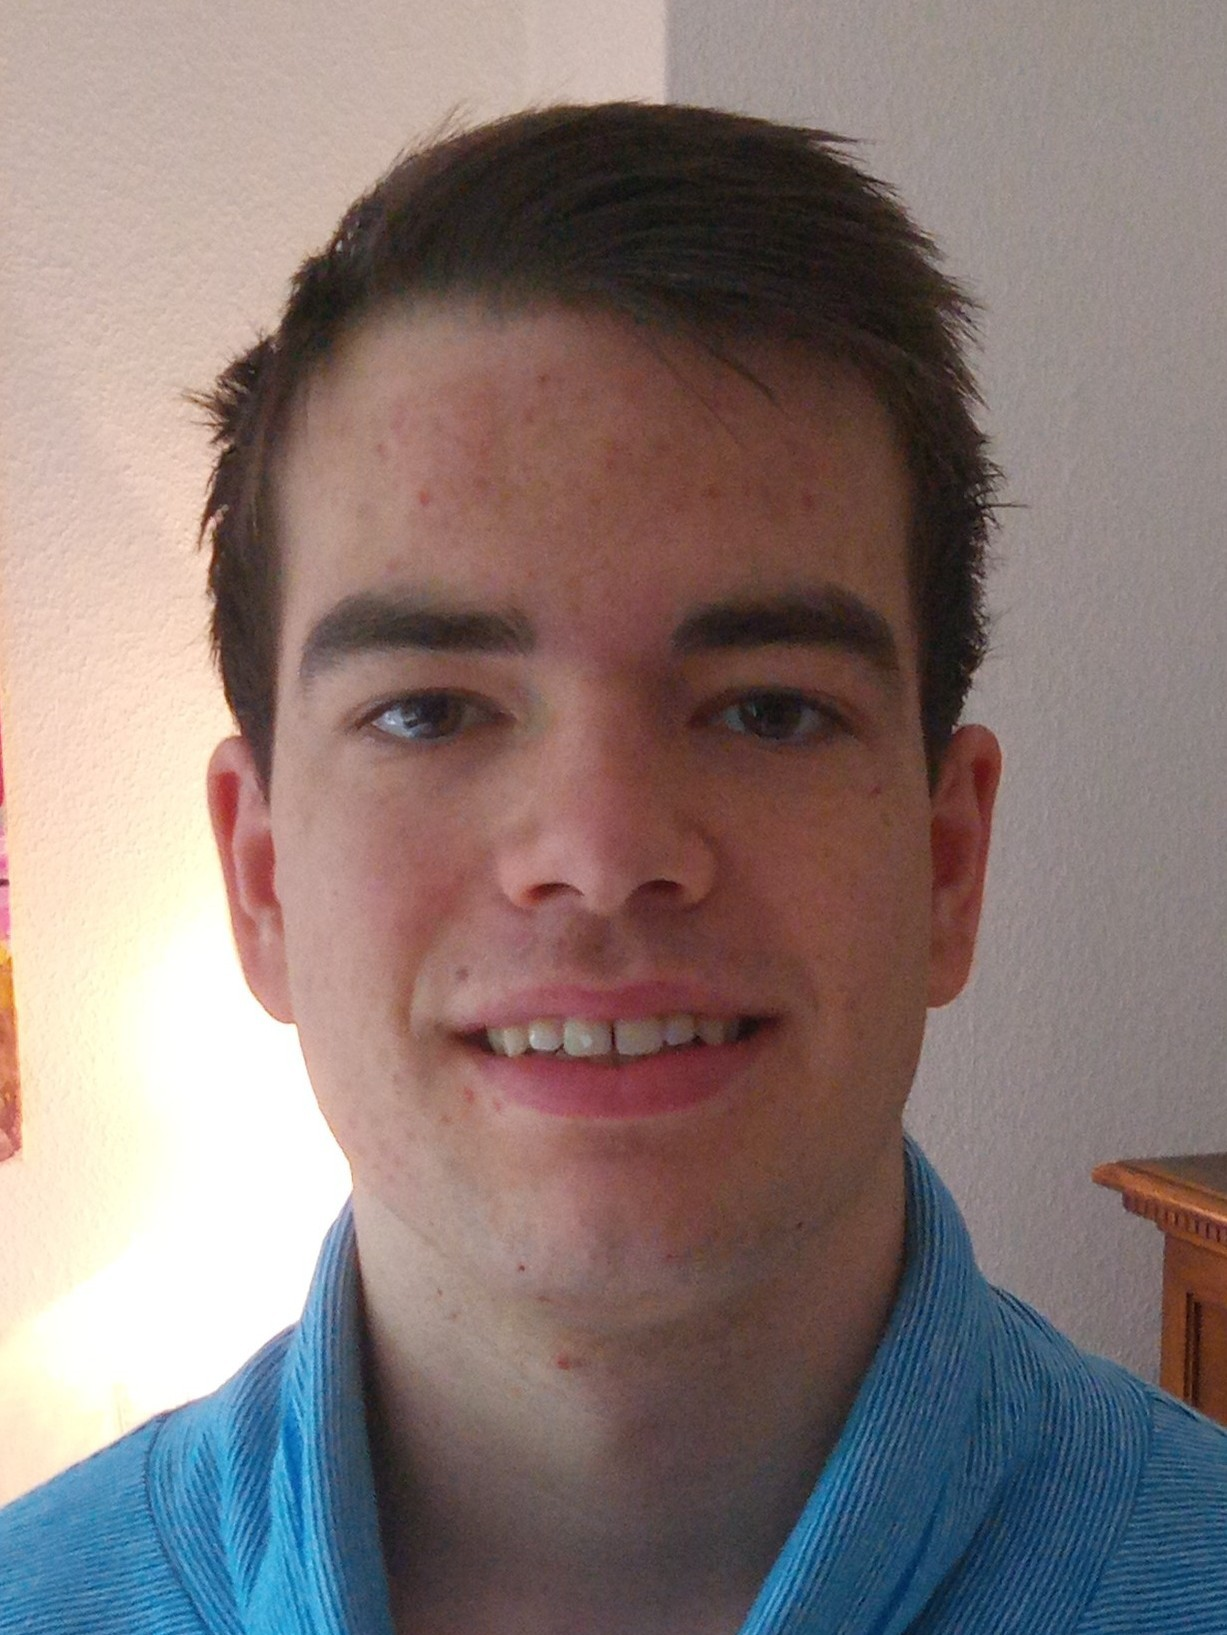
\includegraphics[width=\fibelstdlen]{res/vorstellungsfotos/Fotos Selbstvorstellungstexte Fibel/Lambert.jpg}
	\end{wrapfigure}
}
{
Hallo, ich bin Lambert und fange in diesem Semester meinen Master in Physik an. Aktuell bin ich Vorsitzender der Fachschaft und u.A.\ mitverantwortlich für die Evaluation der Lehre, den BaMa-Tag, die O-Woche und weiß zu viel über Bücher von Neil Gaiman. Mit Fragen zum 1-Fach-Bachelor allgemein und speziell dem Philosophie-Nebenfach sowie allem anderen was euch einfällt, könnt ihr euch gerne an mich wenden. Willkommen in Münster!
}

\vspace{-1.5cm}

\fibelvorstellung{
	\begin{wrapfigure}{r}{0cm}
		\includegraphics[width=\fibelstdlen]{res/vorstellungsfotos/Hauke_neu.jpg}
	\end{wrapfigure}
}
{
Moin, ich heiße Hauke und bin seit 2016 an der Uni und in der Fachschaft. Als Erasmus Student war ich in Sevilla (Spanien) und in Münster bin ich für die Evaluation der Lehre zuständig. Mittlerweile schreibe ich meine Masterarbeit in der Geophysik. 
Euch ein herzliches Willkommen in Münster!
}

\vspace{-2cm}

\fibelvorstellung{
	\begin{wrapfigure}{l}{0cm}
		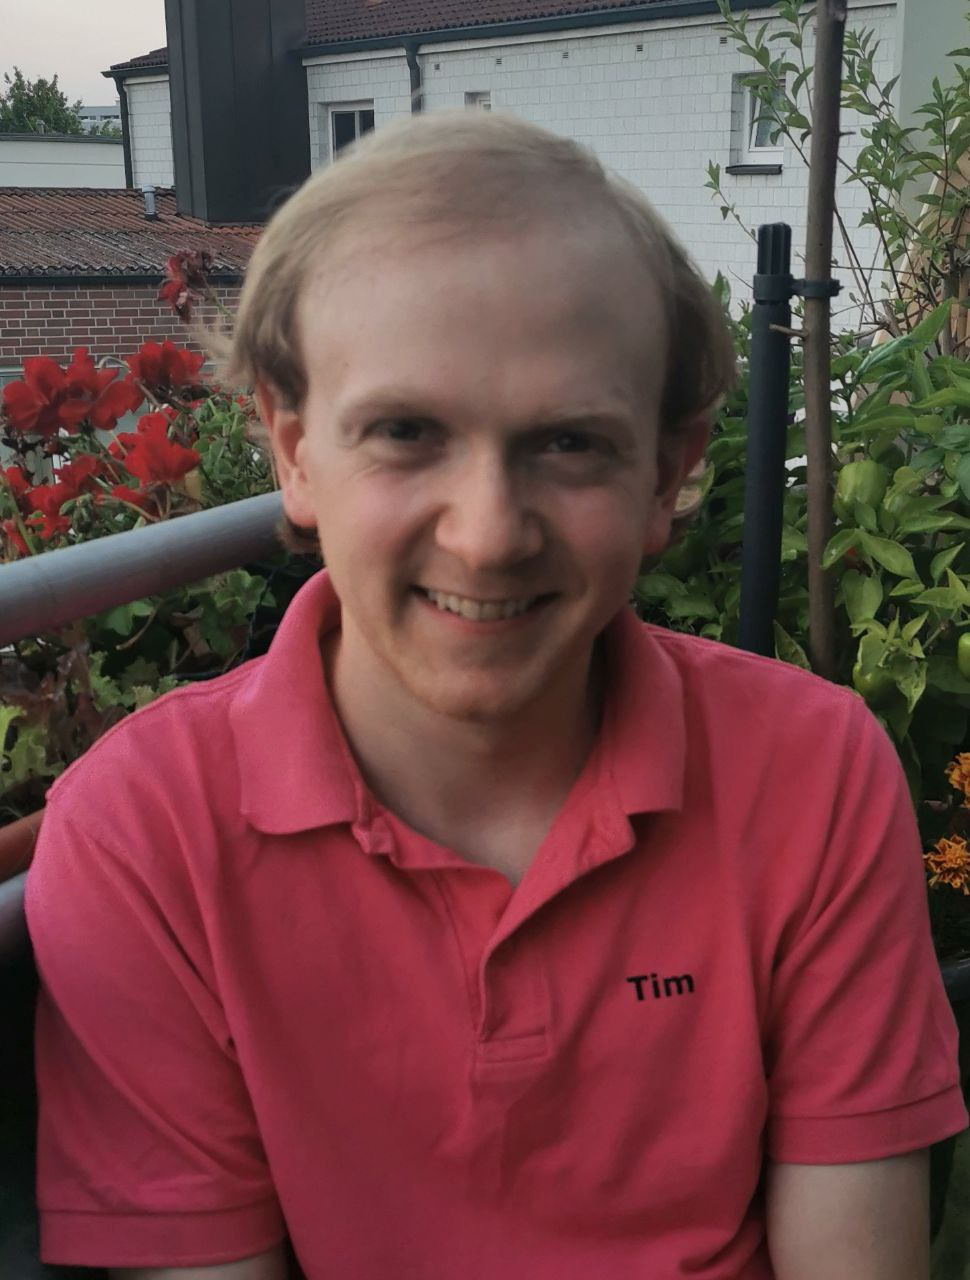
\includegraphics[width=\fibelstdlen]{res/vorstellungsfotos/Tim.jpg}
	\end{wrapfigure}
}
{
Hej, ich bin Tim und studiere Physik im Master. In der Fachschaft bin ich Finanzer, aber auch besonders zu Auslandsaufenthalten kann ich eure Fragen beantworten, denn ich war selber für ein Jahr in Lund in Schweden. 
Für die O-Woche wünsche ich euch viel Spaß und hoffe, dass ihr viele andere Erstis kennen lernt, denn mit Leidensgenossen lassen sich die ganzen Übungszettel deutlich besser rechnen. Doch lasst euch davon nicht abschrecken! Erstmal habt eine schöne Zeit und vielleicht läuft man sich ja mal in der Uni über den Weg, zum Beispiel beim Spieleabend der Fachschaft. ;-)
}

\fibelvorstellung{
	\begin{wrapfigure}{l}{0cm}
		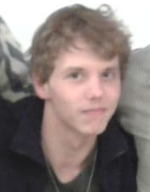
\includegraphics[width=\fibelstdlen]{res/vorstellungsfotos/Marius_cut.PNG}
	\end{wrapfigure}
}
{
Hi, ich bin Marius und heiße euch ebenfalls herzlich willkommen hier in Münster. Wenn ihr die Stadt noch nicht richtig kennt, dann freut euch darauf, sie kennenzulernen. 
Das Studium wird zwar zwischendurch hart, aber lasst euch trotzdem nicht die Freude dran nehmen. ¡Mucha suerte!\footnote{\url{https://www.youtube.com/watch?v=iik25wqIuFo}}
}


\vspace{-0.4cm}

\fibelvorstellung{
	\begin{wrapfigure}{l}{0cm}
		
\includegraphics[width=\fibelstdlen]{res/vorstellungsfotos/Christoph.PNG}
	\end{wrapfigure}
}
{
Sehr geehrte Erstis: Moin!
Ich bin Christoph und studiere im Master Physik. In der Fachschaft bin ich im O-Wochen Team und beim Sommerfest tätig. Wenn Ihr Fragen habt, z.B zur O-Woche oder zum etwas Chaotischen Alltag an der Uni, immer her damit, es lebe das Chaos! :D 
Ich wünsche euch allen eine schöne O-Woche und hoffe man sieht sich mal in der Fachschaft.
}

\vspace{-0.5cm}

\fibelvorstellung{
	\begin{wrapfigure}{r}{0cm}
		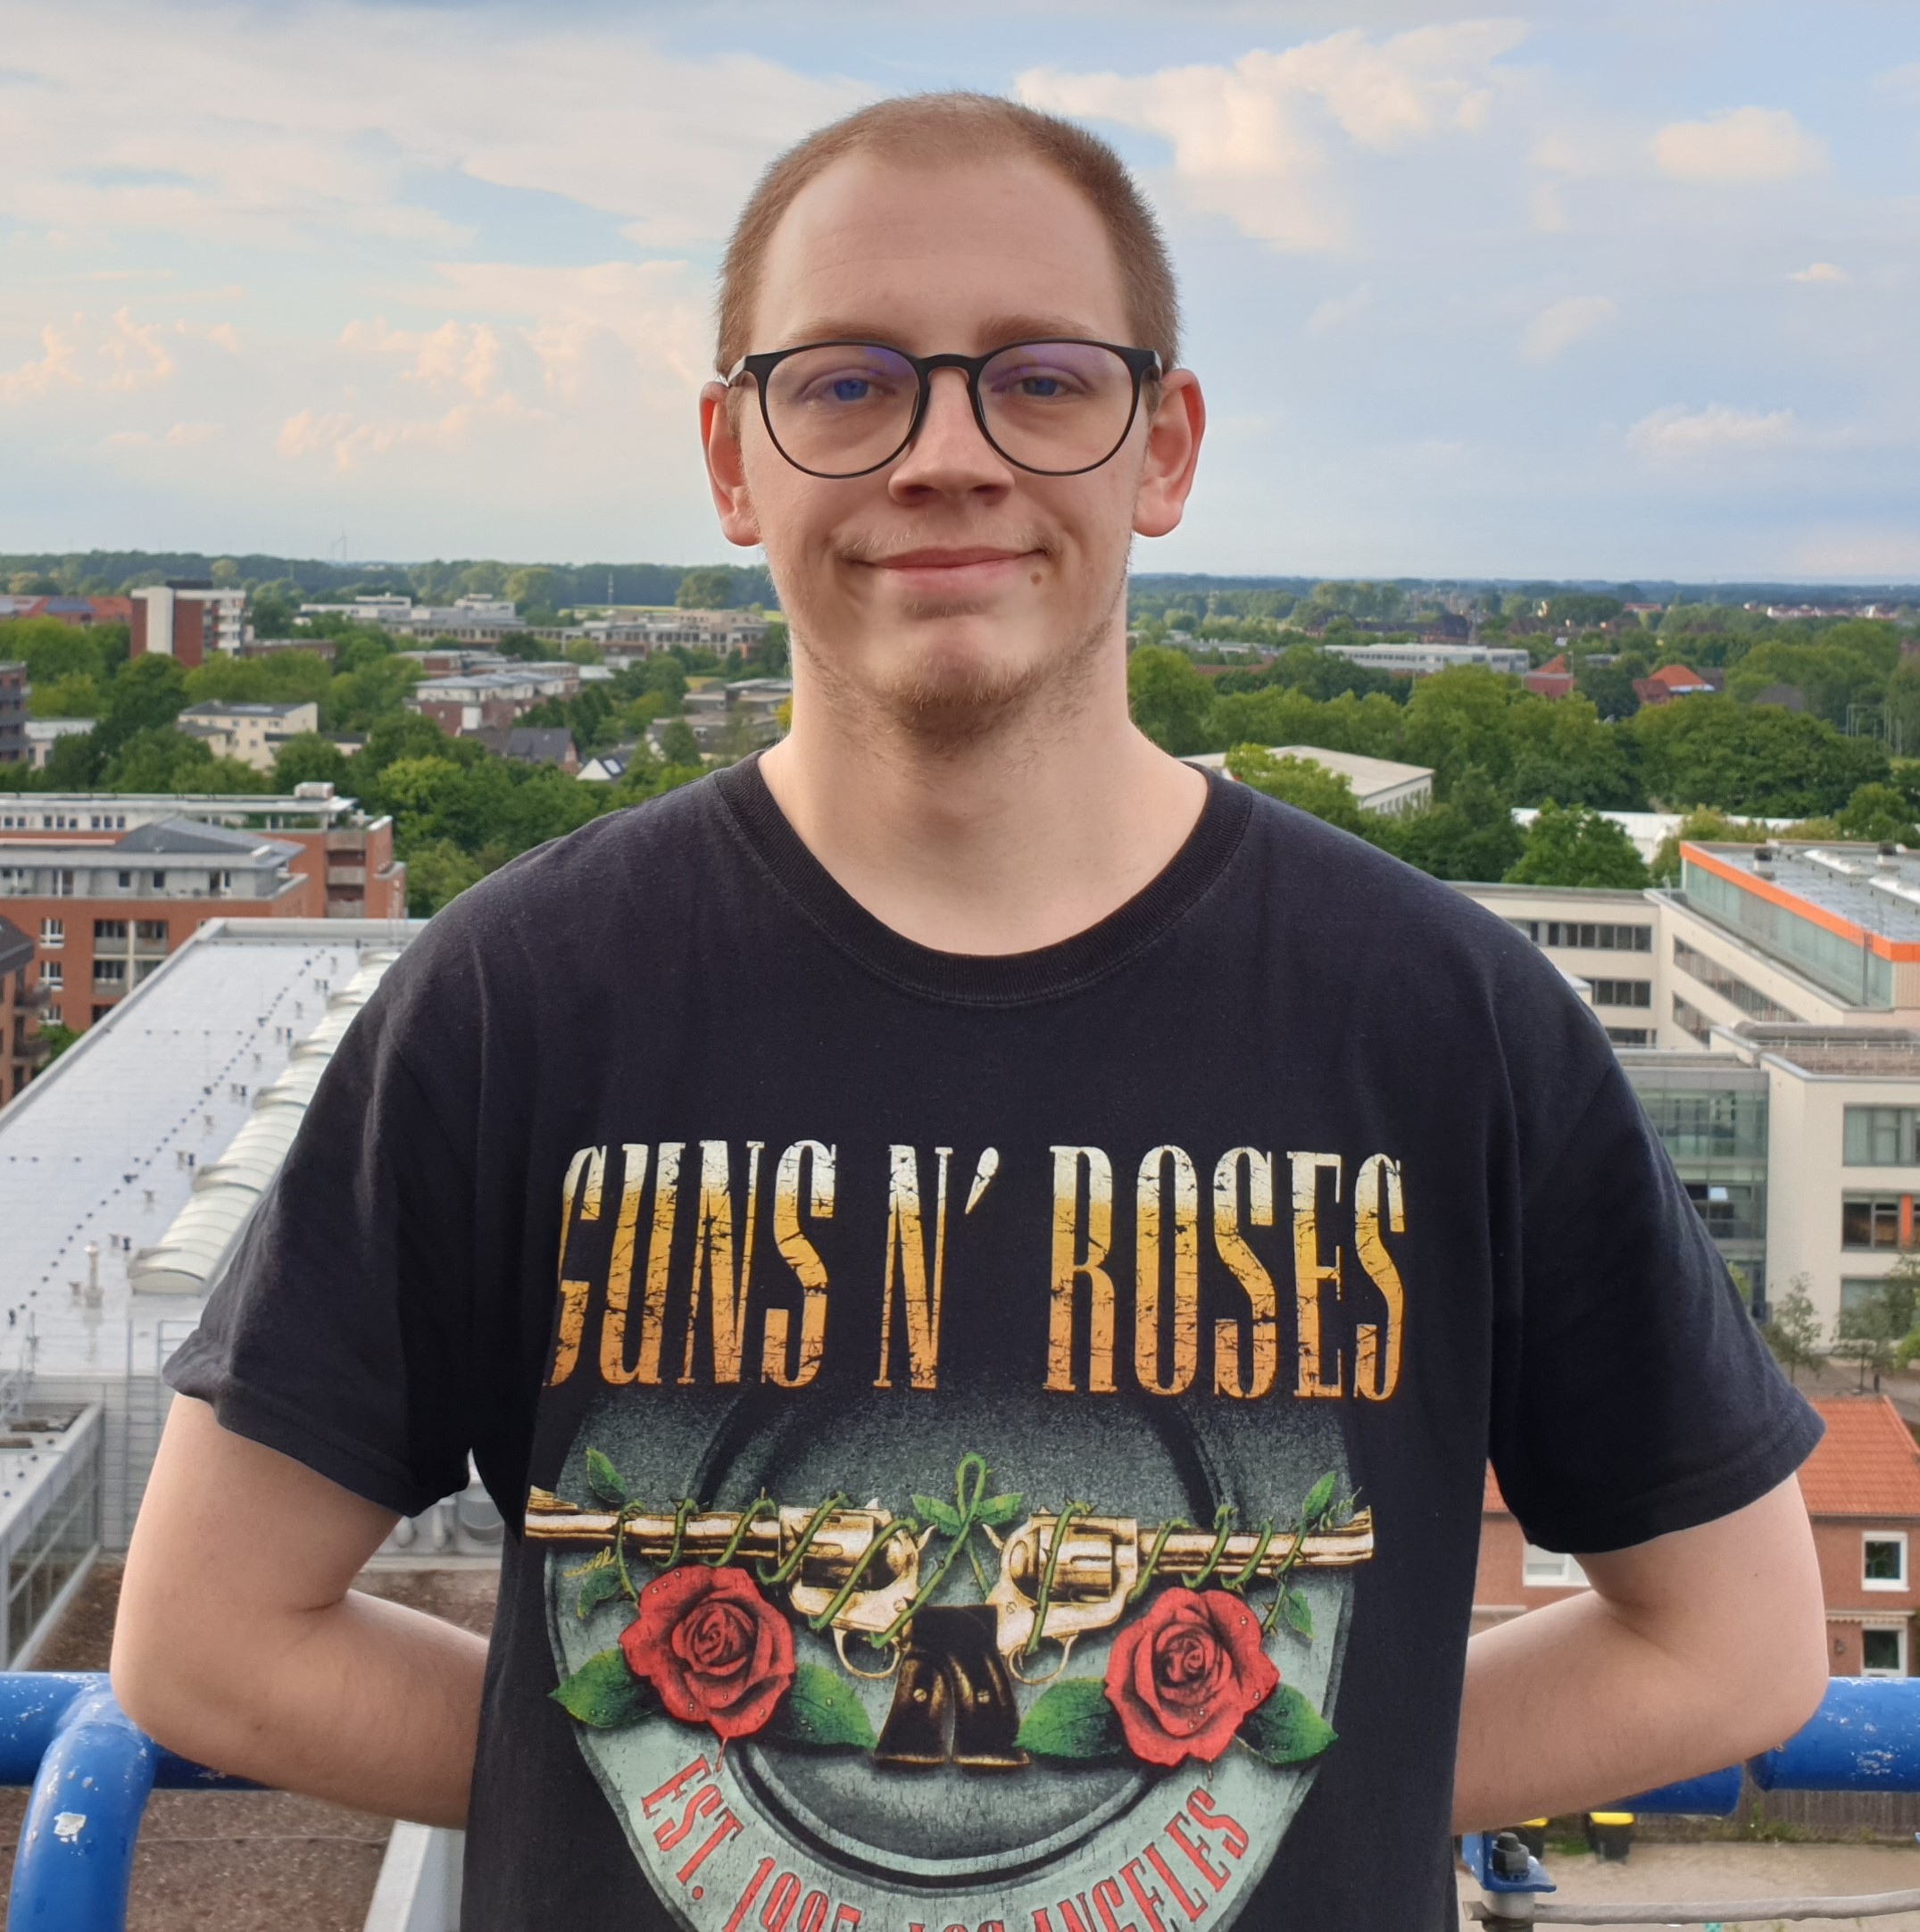
\includegraphics[width=\fibelstdlen]{res/vorstellungsfotos/Alexander_T_cut.jpg}
	\end{wrapfigure}
}
{
Hi, ich bin Alexander und studiere hier Physik im Master. Ich organisiere unter anderem die Ersti-Fahrt, schreibe an dieser Fibel und bin für die IT zuständig. 
Ich heiße euch herzlich willkommen an der Uni Münster und wünsche einen guten Start in das Studium!
}

%\vspace{-1.5cm}

\fibelvorstellung{
	\begin{wrapfigure}{l}{0cm}
		\includegraphics[width=\fibelstdlen]{res/vorstellungsfotos/Jasemin.jpg}
	\end{wrapfigure}
}
{
Hey\textasciicircum\textasciicircum \\
Ich bin Jasemin und studiere Physik und Sozialwissenschaften auf Lehramt. In der Fachschaft bin ich für die O-Woche und die Ersti-Fahrt verantwortlich.
Wenn ihr Fragen zum Lehramt habt, könnt ihr gerne auf mich zukommen.
Ich wünsche euch viel Spaß in eurem Studium.
}

%\vspace{-1.2cm}

\fibelvorstellung{
	\begin{wrapfigure}{l}{0cm}
		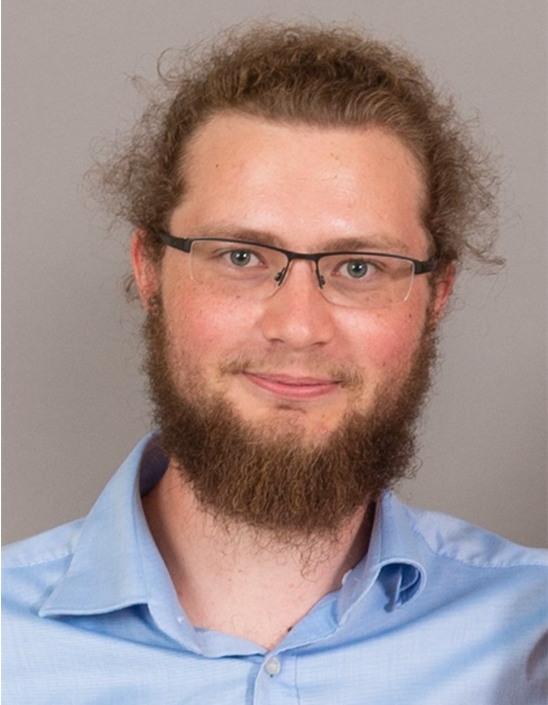
\includegraphics[width=\fibelstdlen]{res/vorstellungsfotos/Ali_cut.PNG}
	\end{wrapfigure}
}
{
Hallo Welt!
Ich verkehre unter den Namen Alexander, Alekschander, Alex, Xander, Ali, Puck, Pucky und dem Akronym APN. Bald ist bei mir die Promotion durch.
In der Fachschaft beschäftige ich mich mit IT-Administration. Entsprechend kann ich bei Fragen zu Physik und Technik gerne helfen.
Forked ruhig meine (Protokoll) Repositories auf GitHub\footnote{\url{https://github.com/APN-Pucky}}.
}

% \vspace{-0.3cm}

\fibelvorstellung{
	\begin{wrapfigure}{l}{0cm}
		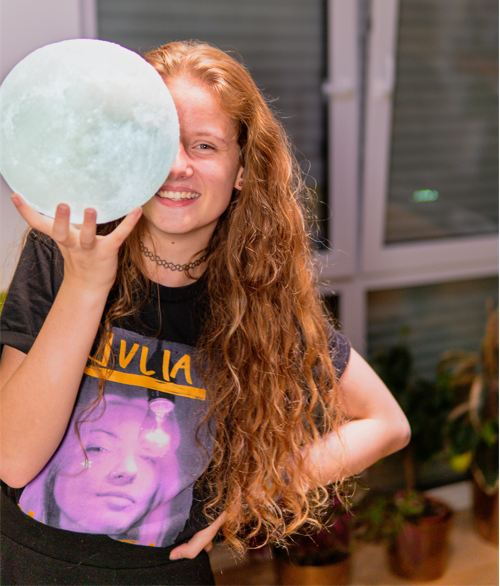
\includegraphics[width=\fibelstdlen]{res/vorstellungsfotos/Eva_cut.PNG}
	\end{wrapfigure}
}
{
Hey, ich heiße Eva und studiere Physik im Master. Seit dem Sommersemester 2020 bin ich in der Fachschaft und betätigte mich im Design-Team und in der Öffentlichkeitsarbeit.
Ich wünsche Euch einen tollen Start ins Studium! PS: Über ein freundliches „Hallo“ (auf dem Gang, im Vorbeigehen) freue ich mich immer.
} 


\fibelvorstellung{
	\begin{wrapfigure}{r}{0cm}
		
\includegraphics[width=\fibelstdlen]{res/vorstellungsfotos/Philipp_cut.JPG}
	\end{wrapfigure}
}
{
Moin! 
Ich bin der Phil, im Moment arbeite ich an meiner Bachelorarbeit sowie ein paar letzten Prüfungen. In der Fachschaft bin ich seit über zwei Jahren aktiv und kümmere mich hier unter Anderem um die Nikolaus-Aktion, im Dezember könnt Ihr diese dann auch bei uns für eure Kommiltionen erwerben. Bis dahin noch eine schöne O-Woche und ein guten Start in das Studium. 
}

%\vspace{0.1cm}

%\vspace{0.1cm}

\fibelvorstellung{
	\begin{wrapfigure}{r}{0cm}
		\includegraphics[width=\fibelstdlen]{res/vorstellungsfotos/Hannes.png}
	\end{wrapfigure}
}
{
Hey, ich bin Hannes und studiere gerade im 3. Semester. Als Nebenfach mache ich Psychologie. In der Fachschaft bin ich unter Anderem bei der Planung des Sommerfests und der Erstifahrt mit eingebunden. Mein Tipp: Sucht euch Leute, mit denen ihr die gemeinsam lernt. Das ist m.M. nach das Wichtigste zum Start! Ansonsten, gebt nicht zu schnell auf. Auch wenn es am Anfang manchmal durchaus frustrierend sein kann.
Falls ihr fragen rund ums Studium habt, sprecht mich gerne an wenn ihr mich seht. :D 
Viel Erfolg!
}

\vspace{-0.3cm}

\fibelvorstellung{
	\begin{wrapfigure}{l}{0cm}
		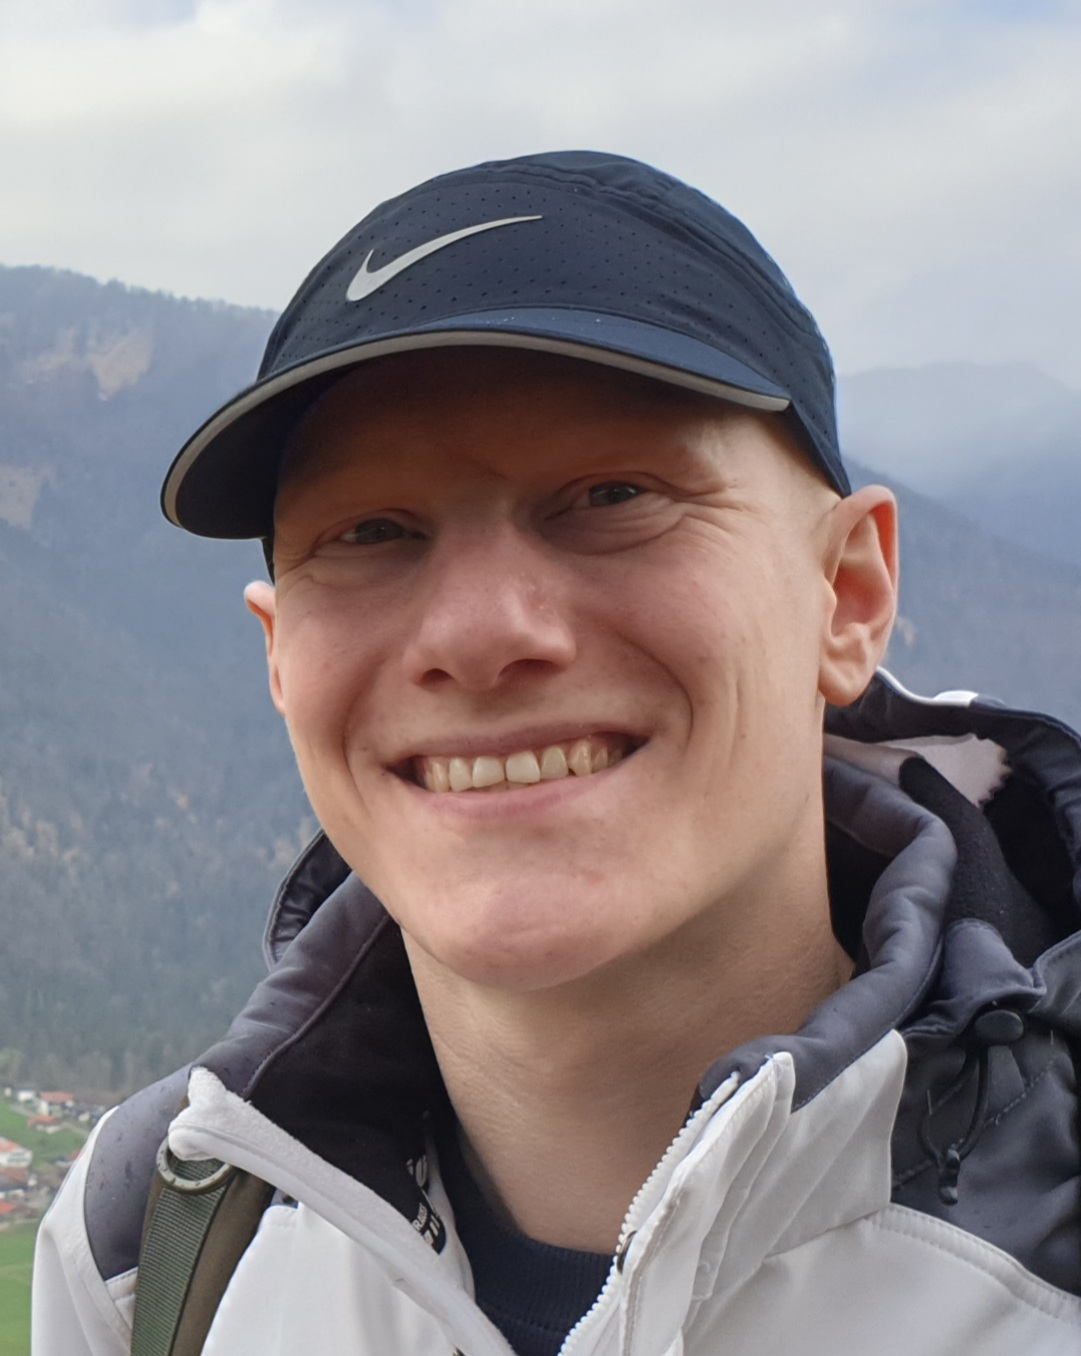
\includegraphics[width=\fibelstdlen]{res/vorstellungsfotos/Marc.jpg}
	\end{wrapfigure}
}
{
Moin! Ich bin Marc und studiere seit 2022 1-Fach Bachelor Physik an der WWU und bin quasi direkt der Fachschaft beigetreten. Ich helfe hier bei der Evaluation der Lehre mit. Mit Fragen könnt ihr sehr gerne zu mir kommen! Insbesondere über mein Nebenfach "Spanisch für Naturwissenschaftler" kann ich euch mittlerweile ein wenig was erzählen. Ich wünsche euch einen tollen Start in euer Studium!!! 
} 

\fibelvorstellung{
	\begin{wrapfigure}{r}{0cm}
		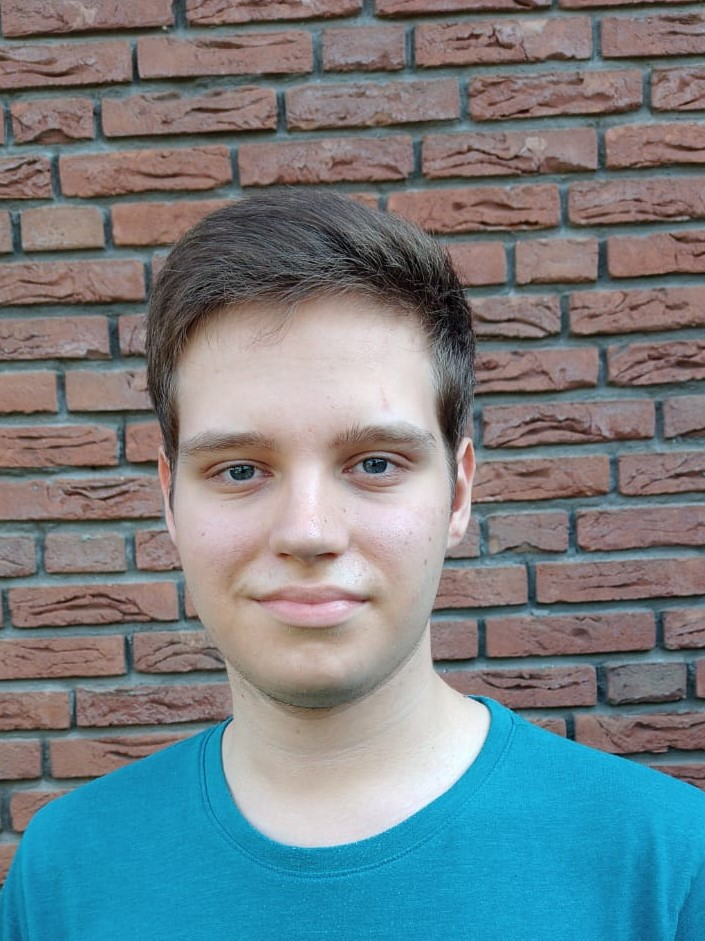
\includegraphics[width=\fibelstdlen]{res/vorstellungsfotos/Phillip_S.jpg}
	\end{wrapfigure}
}
{
Moin, ich bin Phillip und studiere im 3. Semester Physik. In der Fachschaft bin ich für den Hochschultag verantwortlich. Ich wünsche euch eine schöne O-Woche und viel Spaß in Münster und beim Studium. 
}

\fibelvorstellung{
	\begin{wrapfigure}{l}{0cm}
		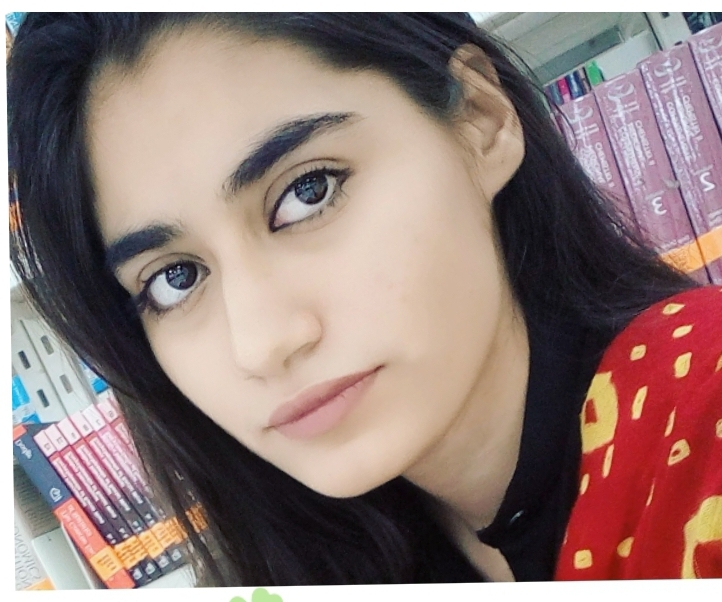
\includegraphics[width=\fibelstdlen]{res/vorstellungsfotos/Saba.jpg}
	\end{wrapfigure}
}
{
Hi, ich bin Saba Ahmed Cheema und studiere Physik auf Master. Zur Zeit bin ich auch Mitglied einer Berufungskommission einer Professur zur Photonik. Ich wünsche euch einen guten Start in's Studium. 
}



%
% \begin{center}
% 	\includegraphics[width=\columnwidth]{res/fsphys_logo.pdf}
% \end{center}
%
%
%

% \vspace{6ex}

% \fibelvorstellung{
% 	\begin{wrapfigure}{r}{0cm}
% 		\includegraphics[width=\fibelstdlen]{res/vorstellungsfotos/fritz.png}
% 	\end{wrapfigure}
% }
% {
% Hallo, ich bin Fritz und bin schon  in der Fachschaft Physik.
% Die Mannschaft hier ist echt genial aufgestellt. Dadurch macht es richtigen Spaß, ein aktiver Teil der Universität % Münster zu sein.
% Ich kann dir nur empfehlen: Mach' mit und verändere die Uni!
% }


\end{multicols}

% \vspace{20ex}
